%   ------------------------------------------------------------------------
\FloatBarrier
\section{Análise do CGDream}
\label{s.CGDream}

A ferramenta CGDream foi selecionada por sua capacidade de gerar imagens a partir de uma referência e uma descrição textual, com o objetivo de criar uma imagem do personagem Pablo em side view a partir de sua arte em front view (apresentada anteriormente na Figura \ref{fig:Pablo}). A lógica por trás disso é que essa imagem possa ser usada também de referência para a animação. A plataforma se destaca pela vasta gama de opções de customização, porém apresenta uma interface visualmente poluída, o que pode dificultar a localização de suas funcionalidades (Figura \ref{fig:CGDreamTela} no Apêndice \ref{ap.telasIA}).

A ferramenta permite o envio de uma referência e oferece múltiplos modos de uso para essa imagem (Figura \ref{fig:CGDreamOpcoes} no Apêndice \ref{ap.telasIA}):

\begin{itemize}
    \item Estilo de referência, manter o estilo;
    \item Estrutura de referência, pegar uma estrutura, como construções;
    \item Imagem como referência, usar uma figura como referência para a geração;
    \item 3D para imagem, transformar um modelo 3D em uma imagem; e
    \item Personagem consistente, reconhecer um personagem e usar como guia para a geração.
\end{itemize}


Em relação a todas as outras ferramentas, o site possui uma interface extremamente poluída, como pode ser visto na Figura \ref{fig:CGDreamTela}, ficando até difícil localizar todos os elementos. Na parte inferior, tem a área para escrever o prompt, podendo selecionar filtros baseados em imagens pela própria plataforma para direcionar a geração. No canto esquerdo, é possível anexar uma referência e selecionar a força que ela vai ter para mudar a geração. Essa  imagem pode ser usada de diferentes formas dependendo da opção selecionada : 

A plataforma também possui outras opções de customização, como filtros específicos para direcionar a geração, uma variável chamada prompt guidance (orientação do prompt) e dois modelos de IA: o Juggernaut XL, ideal para fotorrealismo de acordo com \cite{xu_cohen_clark_2025}, e o Flux, conhecido por sua alta fidelidade aos prompts \cite{greenberg} e o mais recomendado para uso \cite{cgdream_video}.

A análise foi focada em duas funcionalidades principais: Imagem como referência e Personagem consistente.

Os testes direcionados à funcionalidade Imagem como referência apresentaram resultados interessantes, comparando o desempenho dos modelos Flux e Juggernaut XL.

Na primeira interação, foi selecionado o modelo Flux no modo Dev, com o prompt "boy facing east" (menino voltado para o leste, em português). Os resultados apresentados apresentavam uma semelhança média com a referência e mantiveram o estilo pixel art 2D, porém o personagem foi gerado em front view, e em uma das imagens ele apenas movia os olhos para a esquerda. Analisando esses dados, a ferramenta parece ter interpretado o prompt como se o personagem devesse estar olhando para a esquerda com apenas os olhos, sem o corpo estar virado. Interação completa pode ser consultada na Figura \ref{fig:cgDream1} no Apêndice \ref{ap.telasIA}.

Na segunda interação, foi selecionado o modelo Juggernaut XL no modo Quality, mantendo o exato mesmo prompt para fins de comparação com o resultado anterior. As imagens geradas mantiveram o ambiente 2D e apresentaram semelhanças médias com a imagem de referência, porém o estilo de pixel art não foi incorporado de maneira satisfatória e também ignorou a instrução textual. Por esse motivo, outro teste foi realizado aumentando o valor de prompt guidance, o que melhorou a fidelidade do estilo, porém não corrigiu a pose. A interação completa é mostrada nas Figuras \ref{fig:cgDream2} e \ref{fig:cgDreamJugger8} no Apêndice \ref{ap.telasIA}. 

A Figura \ref{fig:cgDreamMelhorImagem}compara o melhor resultado obtido em cada um dos testes. Embora o modelo Flux tenha sido superior na manutenção do estilo, nenhum dos resultados foi consistente o suficiente para uso no jogo, e o objetivo principal (gerar o personagem em side view) não foi alcançado. Adicionalmente, nenhuma das imagens geradas atingiu um padrão pixel perfect (Figura \ref{fig:CGDreamPixelPerfect}).


\begin{figure}[htbp]
    \centering
    \caption{\small Melhores resultados do CGDream utilizando a funcionalidade de imagem}
    \label{fig:cgDreamMelhorImagem}
    \begin{subfigure}{0.21\linewidth}
        
\includegraphics[width=1\linewidth]{figs/sprites/Pablo.PNG}
        \caption{\small Imagem de referência}
        \label{fig:CGDreamPablo}
    \end{subfigure}
    \begin{subfigure}{0.21\linewidth}
        
\includegraphics[width=1\linewidth]{figs/cgDream/res_img_fluxDev1b.png}
        \caption{\small Melhor resultado Flux}
        \label{fig:cgDreamMelhorImagemFlux}
    \end{subfigure}
    \begin{subfigure}{0.21\linewidth}
        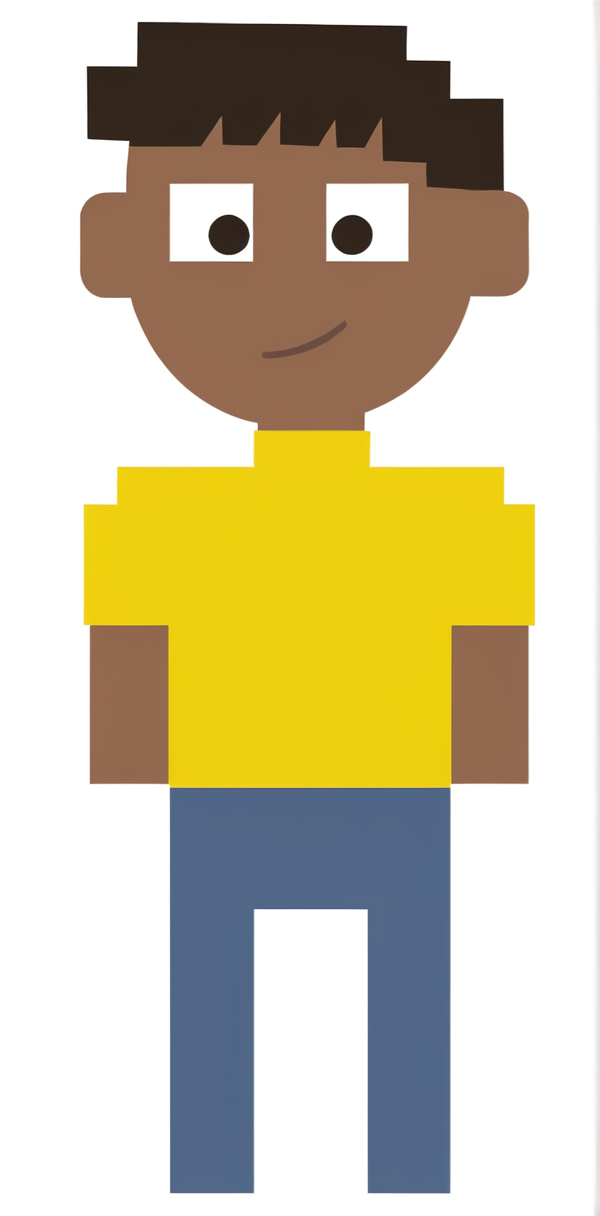
\includegraphics[width=1\linewidth]{figs/cgDream/res_img_jug2b.png}
        \caption{\small Melhor resultado Juggernaut XL com prompt guidance 5}
        \label{fig:cgDreamMelhorImagemJug}
    \end{subfigure}
    \begin{subfigure}{0.21\linewidth}
        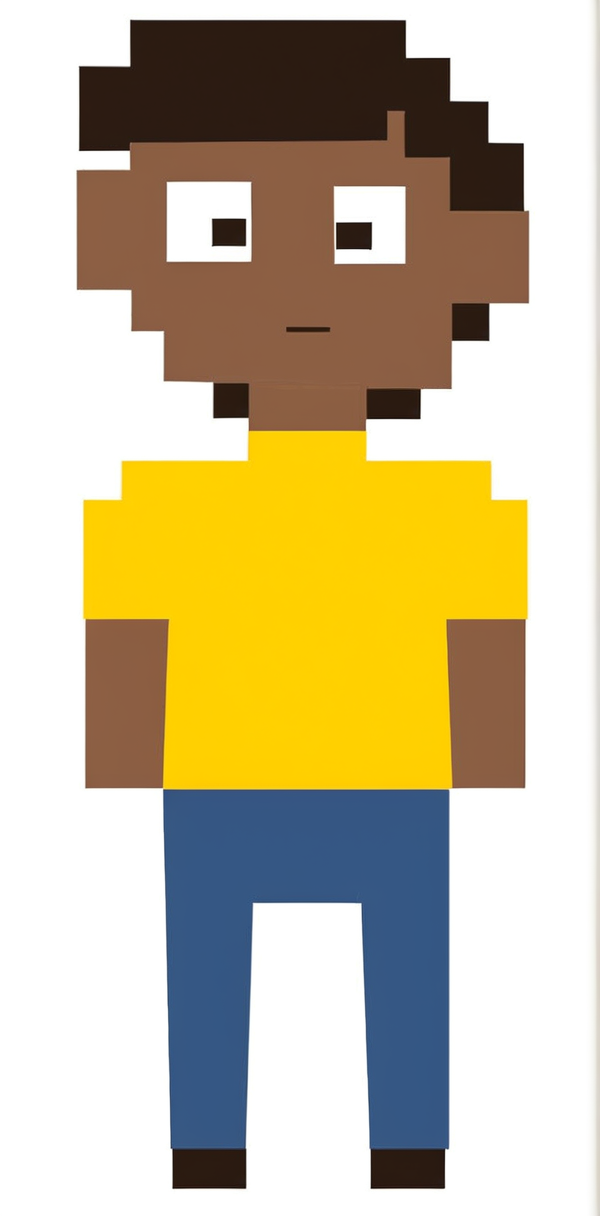
\includegraphics[width=1\linewidth]{figs/cgDream/res_img_jug8a.png}
        \caption{\small Melhor resultado Juggernaut XL com prompt guidance 8}
        \label{fig:cgDreamMelhorImagemJug8}
    \end{subfigure}

    \legend{\small Fonte: Elaborada pela autora, utilizando a ferramenta CGDream.}
\end{figure}

\begin{figure}[htbp]
    \centering
    \caption{\small Pixels de tamanho diferente}
    \label{fig:CGDreamPixelPerfect}
    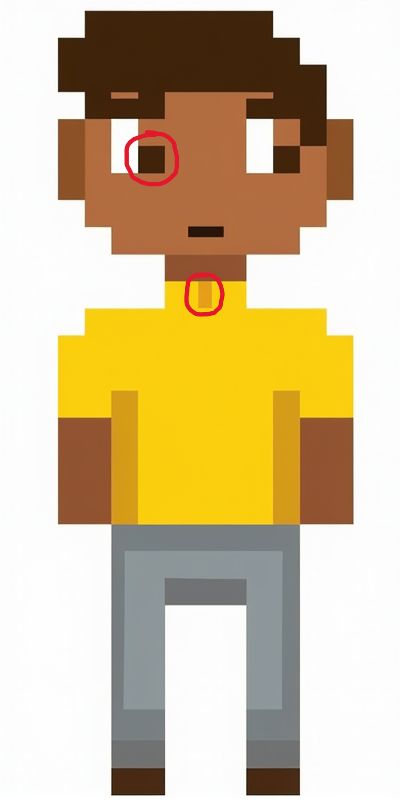
\includegraphics[width=0.3\linewidth]{figs/cgDream/pixel perfect.png}
    \legend{\small Fonte: Elaborada pela autora.}
\end{figure}

Em testes posteriores voltados para o modelo Flux, com prompts ajustados para especificar melhor a pose, a ferramenta não apresentou resultados melhores, continuando a ignorar a instrução textual, apesar de gerar um personagem consistente. Analisando os resultados, é possível perceber que a funcionalidade Imagem como referência desenha a nova figura de maneira a continuar semelhante à figura enviada, mesmo que tenha que ignorar o prompt para isso. Esses testes podem ser consultados nas Figuras \ref{fig:cgDream3} e \ref{fig:cgDream4} no Apêndice \ref{ap.telasIA}. Devido a nenhum dos resultados ter sido satisfatório, essa funcionalidade é descartada.

Os testes direcionados à funcionalidade Personagem consistente apresentaram resultados insatisfatórios. 


Seguindo a mesma lógica das interações com a imagem de referência, primeiro foi selecionado o modelo Flux Dev e depois o Juggernaut XL, ambos com o mesmo prompt: "boy facing east". A ferramenta ignorou completamente a imagem de referência, gerando personagens, estilos e cenários totalmente novos, apenas cumprindo de maneira parcial a instrução da pose. Mais algumas tentativas foram feitas, ajustando o prompt e usando a funcionalidade de filtro e de palavras negativas (exclusivo do modelo Juggernaut XL que permite especificar o que é para ser evitado na geração), o que gerou a pose precisa, porém manteve os problemas de consistência. O processo completo pode ser consultado na \ref{fig:cgDream5} a \ref{fig:cgDream7} do Apêndice \ref{ap.telasIA}.

Uma nova estratégia foi implementada, combinando a funcionalidade Personagem Consistente com a de Estilo de Referência, utilizando a mesma imagem em ambas. visando explorar as outras funcionalidades do site. Além disso, a funcionalidade de filtro também foi usada para especificar a imagem em pixel art e o prompt foi ajustado para descrever o personagem, visto que os resultados anteriores não mantiveram nenhuma característica da referência. As interações completas podem ser encontradas nas Figuras \ref{fig:cgDream8} e \ref{fig:cgDream9}.

Essa abordagem se mostrou mais eficaz em manter as características do personagem original, como pode ser observado nas Figuras \ref{fig:cgDreamPersonagemComparaFlux} e \ref{fig:cgDreamPersonagemComparaJug}.

\begin{figure}[htbp]
    \centering
    \caption{\small Comparativo de resultados do modelo Flux com e sem Estilo de referência}
    \label{fig:cgDreamPersonagemComparaFlux}
    \begin{subfigure}{0.45\linewidth}
        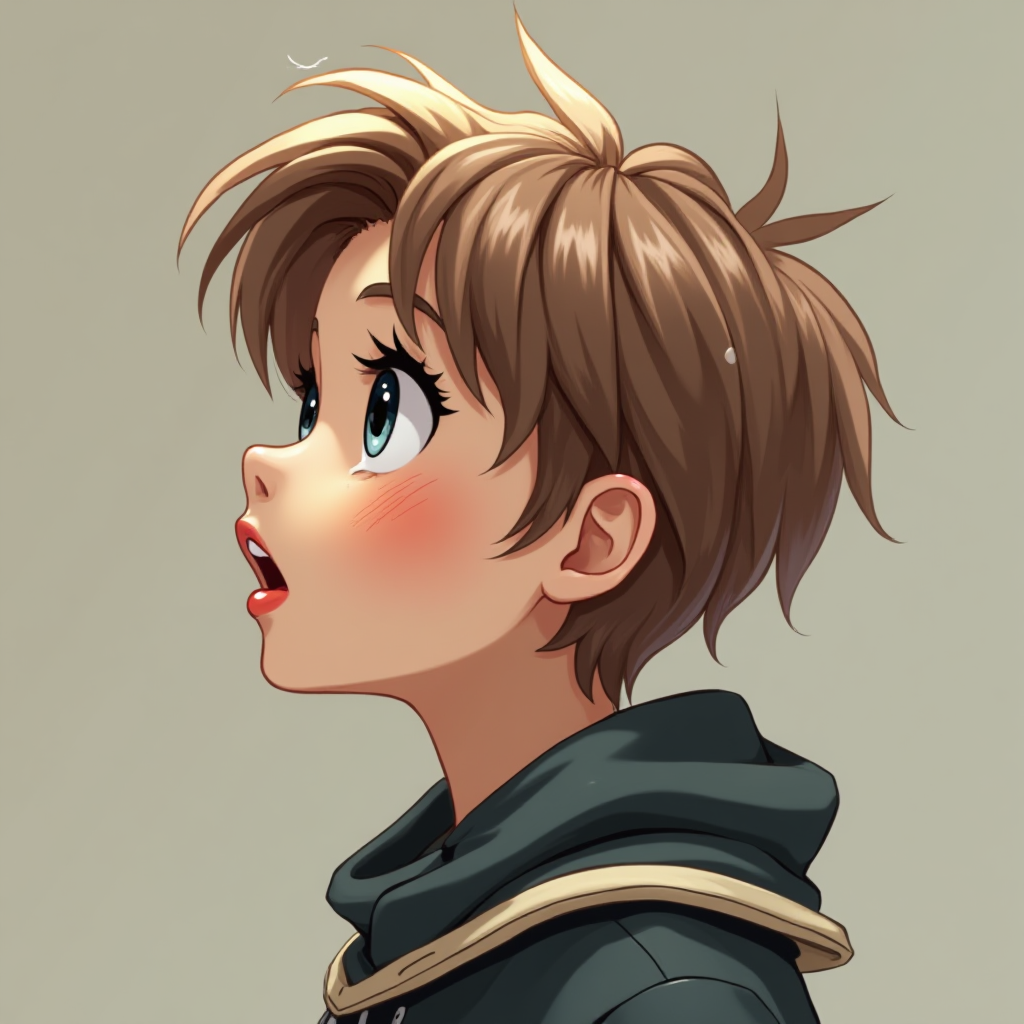
\includegraphics[width=1\linewidth]{figs/cgDream/res_char_fluxFast1.png}
        \caption{\small Imagem gerada apenas utilizando personagem de referência}
        \label{fig:CGDreamFluxSemEstilo}
    \end{subfigure}
    \begin{subfigure}{0.45\linewidth}
        
\includegraphics[width=1\linewidth]{figs/cgDream/res_char_FluxFast_filtro2.png}
        \caption{\small Imagem gerada usando personagem e estilo de referência}
        \label{fig:cgDreamFluxComEstilo}
    \end{subfigure}
    \legend{\small Fonte: Elaborada pela autora, utilizando a ferramenta CGDream.}
\end{figure}

\begin{figure}[htbp]
    \centering
    \caption{\small Comparativo de resultados do modelo Juggernaut XL com e sem Estilo de referência}
    \label{fig:cgDreamPersonagemComparaJug}
    \begin{subfigure}{0.45\linewidth}
        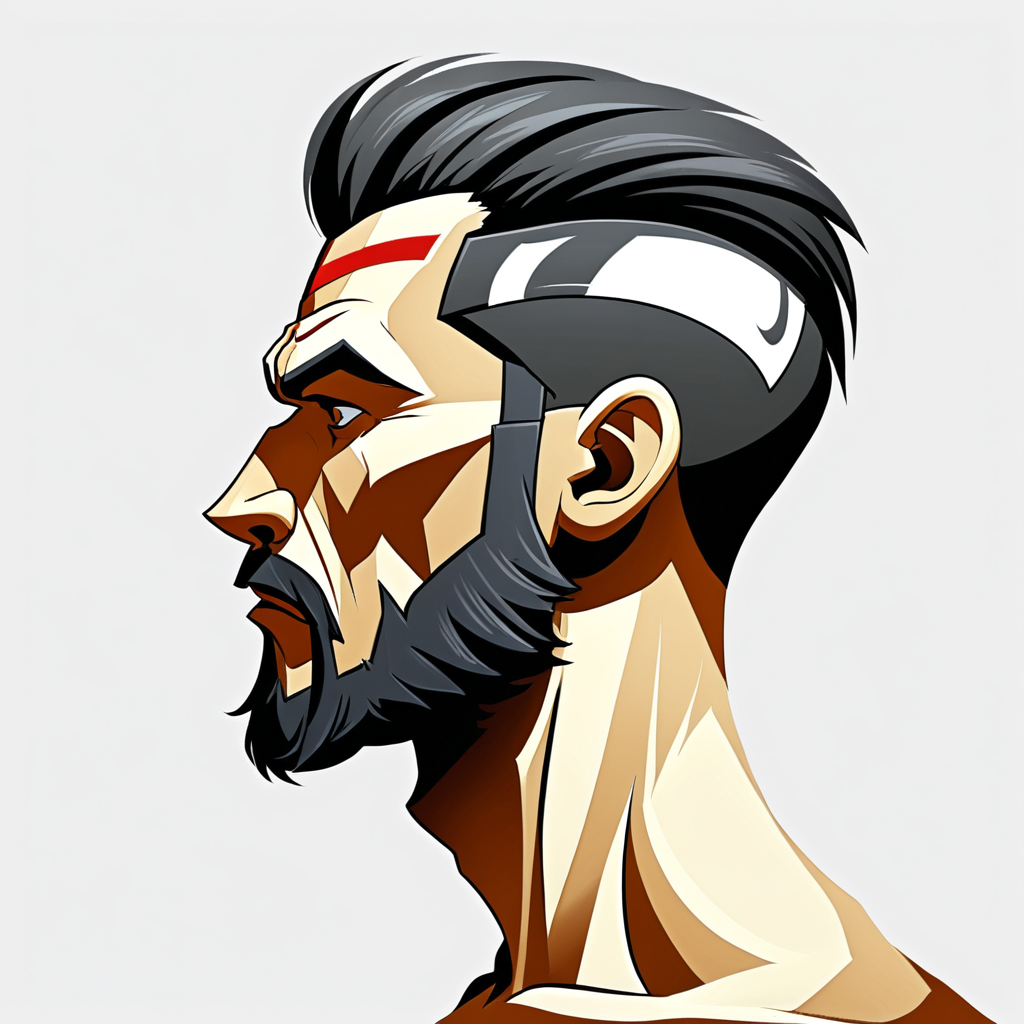
\includegraphics[width=1\linewidth]{figs/cgDream/res_char_jug8.png}
        \caption{\small Imagem gerada apenas utilizando personagem de referência}
        \label{fig:CGDreamJugSemEstilo}
    \end{subfigure}
    \begin{subfigure}{0.45\linewidth}
        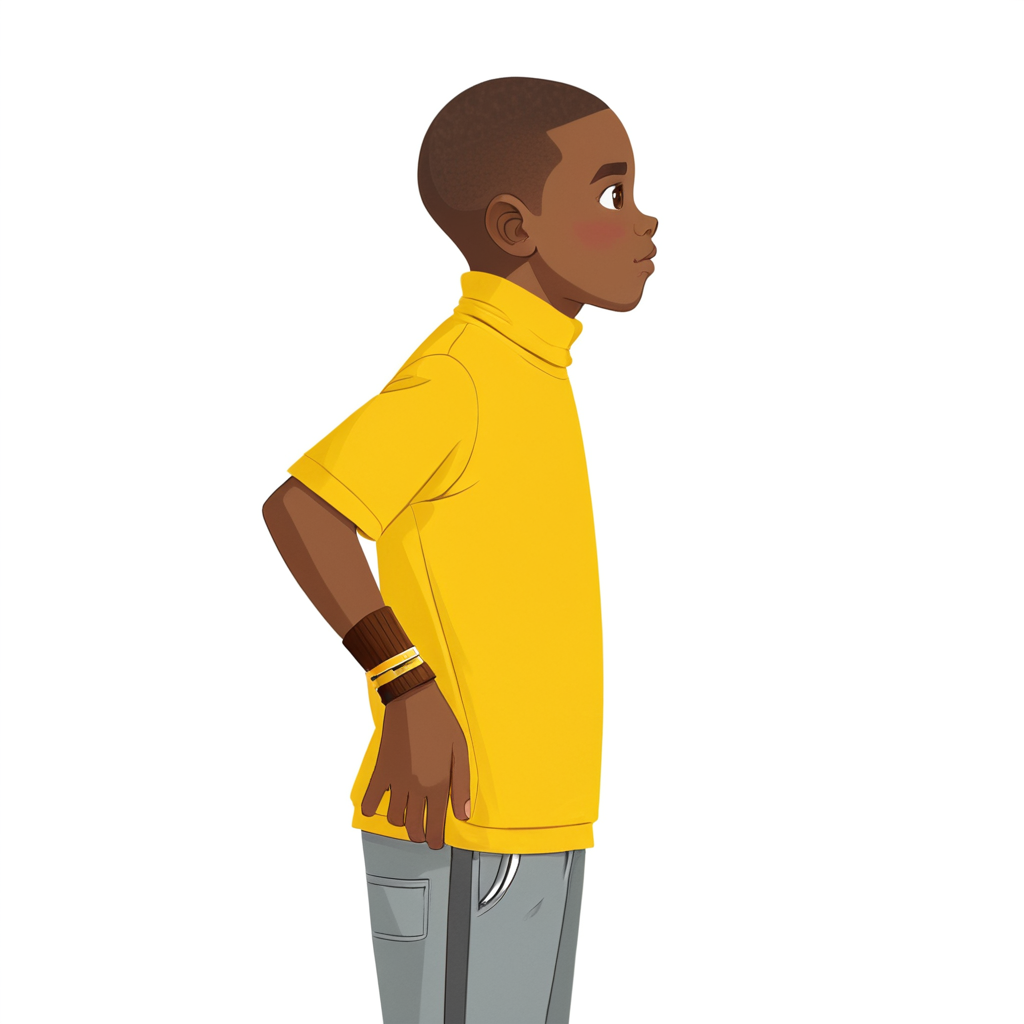
\includegraphics[width=1\linewidth]{figs/cgDream/res_char_jug_estilo1c.png}
        \caption{\small Imagem gerada usando personagem e estilo de referência}
        \label{fig:cgDreamJugComEstilo}
    \end{subfigure}
    \legend{\small Fonte: Elaborada pela autora, utilizando a ferramenta CGDream.}
\end{figure}

Apesar da melhora na consistência, novos problemas surgiram. O modelo Flux passou a gerar imagens borradas e com a pose de costas. Esse problema ocorre independentemente do prompt ou filtro usado, como é demonstrado na Figura \ref{fig:cgDreamPersonagemPadraoFluxEstilo}. O modelo Juggernaut XL, por sua vez, gerava imagens no estilo realista quando "3D" como palavra negativa não era explicitamente utilizada, indicando que a referência de estilo era usada apenas para capturar as características do personagem, não sua estética pixel art (como pode ser observado na Figura \ref{fig:cgDreamPersonagemComparaJugPalavra}).

\begin{figure}[htbp]
    \centering
    \caption{\small Comparativo de resultados do modelo Flux com e sem filtro pixelizado}
    \label{fig:cgDreamPersonagemPadraoFluxEstilo}
    \begin{subfigure}{0.45\linewidth}
        
\includegraphics[width=1\linewidth]{figs/cgDream/res_char_FluxFast_estilo1.png}
        \caption{\small Imagem gerada sem utilizar filtro pixelado}
        \label{fig:CGDreamFluxEstiloSemFiltro}
    \end{subfigure}
    \begin{subfigure}{0.45\linewidth}
        
\includegraphics[width=1\linewidth]{figs/cgDream/res_char_FluxFast_filtro1.png}
        \caption{\small Imagem gerada usando filtro pixelado}
        \label{fig:cgDreamFluxEstiloComFiltro}
    \end{subfigure}
    \legend{\small Fonte: Elaborada pela autora, utilizando a ferramenta CGDream.}
\end{figure}

\begin{figure}[htbp]
    \centering
    \caption{\small Comparativo de resultados do modelo Juggernaut XL com e sem Estilo de referência}
    \label{fig:cgDreamPersonagemComparaJugPalavra}
    \begin{subfigure}{0.45\linewidth}
        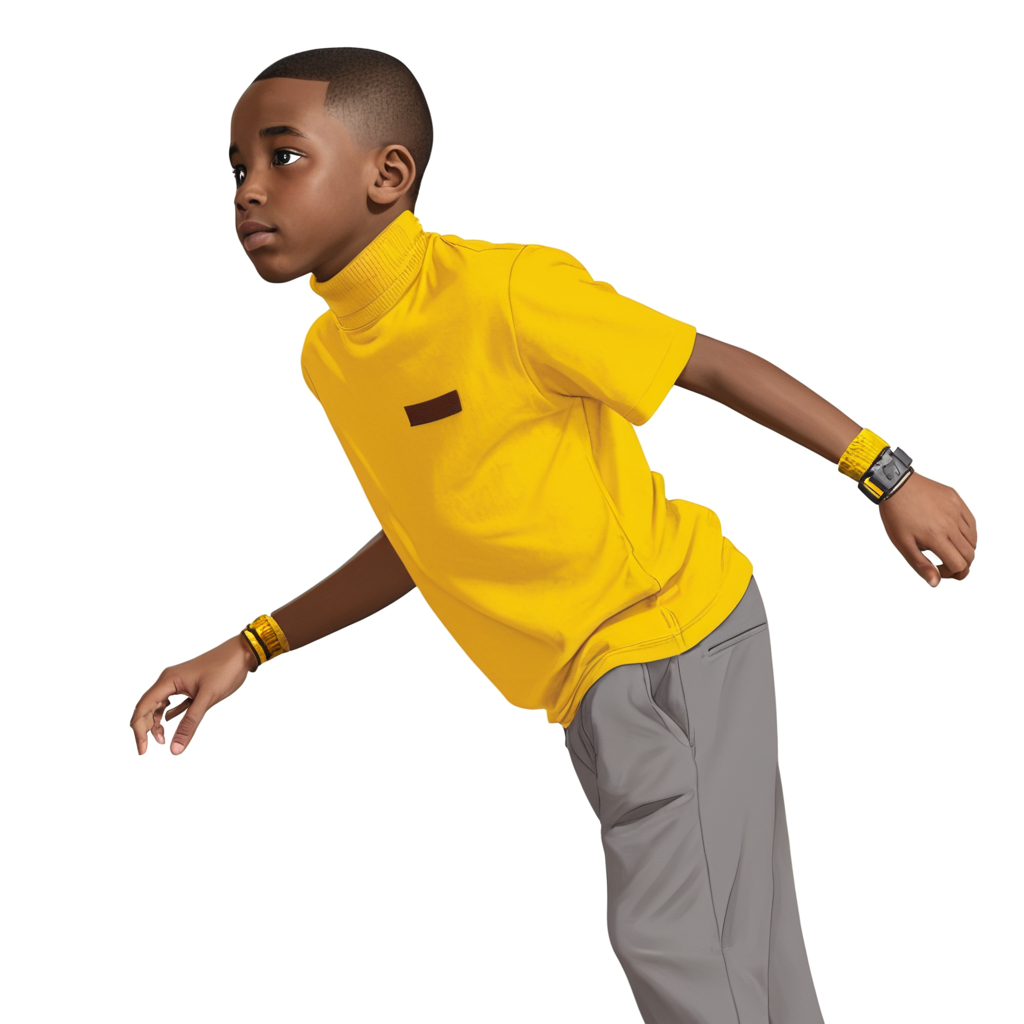
\includegraphics[width=1\linewidth]{figs/cgDream/res_char_jug_estilo1b.png}
        \caption{\small Imagem gerada com apenas "blur" como palavra negativa}
        \label{fig:CGDreamJugSemNegativo}
    \end{subfigure}
    \begin{subfigure}{0.45\linewidth}
        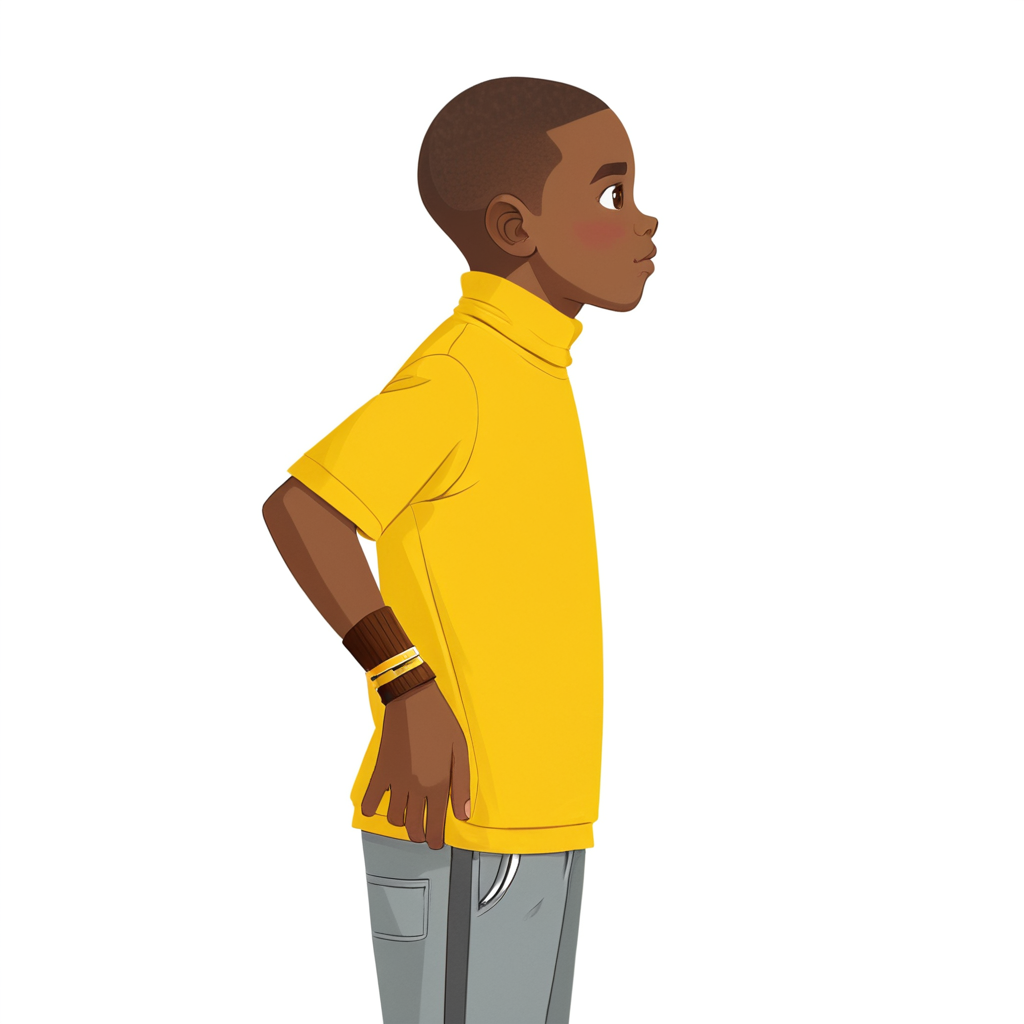
\includegraphics[width=1\linewidth]{figs/cgDream/res_char_jug_estilo1c.png}
        \caption{\small Imagem gerada com "3D" e "blur" como palavras negativas}
        \label{fig:cgDreamJugComNegativo}
    \end{subfigure}
    \legend{\small Fonte: Elaborada pela autora, utilizando a ferramenta CGDream.}
\end{figure}

Após uma extensa bateria de testes, conclui-se que a ferramenta CGDream, apesar de seu potencial e complexidade, não é adequada para a tarefa de gerar sprites consistentes para um jogo já em desenvolvimento. Ambas as funcionalidades testadas falharam em um ou mais critérios essenciais: manter o estilo pixel art, reproduzir fielmente o design do personagem ou seguir a instrução de pose do prompt. Portanto, a ferramenta foi descartada.